% vim:set spell:
% vim:spell spelllang=fr:
\documentclass[a4paper]{article}
\usepackage[utf8x]{inputenc}
\usepackage[T1]{fontenc}
\usepackage{libertine}
\usepackage{helvet}
\usepackage{graphicx}
\usepackage{amsmath,amssymb}
\usepackage[french]{babel}
\usepackage{xspace}
\usepackage{setspace}
\setstretch{1.0}
\usepackage{subfigure}
\usepackage{listings}
\voffset       -1in
\hoffset       -1in
\headheight     12pt
\headsep        12pt
\topmargin      25mm
\oddsidemargin  20mm
\textwidth      170mm
\textheight     240mm
\flushbottom
\lstset{numbers=left, numberstyle=\tiny, stepnumber=1, numbersep=5pt}
\graphicspath{{../../scripts/}}
\begin{document}
\begin{center}
\large
Travaux Pratiques Archi SEOC-3A\\
\LARGE
Prédiction de branchements\\
\large

\end{center}
\section{Identification}
Travail réalisé par Frédéric Pétrot

\section{Prédicteur $n$ modal : conception et résultats}
\subsection{Conception}
Le prédicteur $n$ modal bit est constitué d'un unique tableau contenant de $2^1$ à $2^3$ bits.

\subsection{Résultats}
Les résultats issus de la simulation sont les suivants.
\par
\begin{minipage}{.48\linewidth}
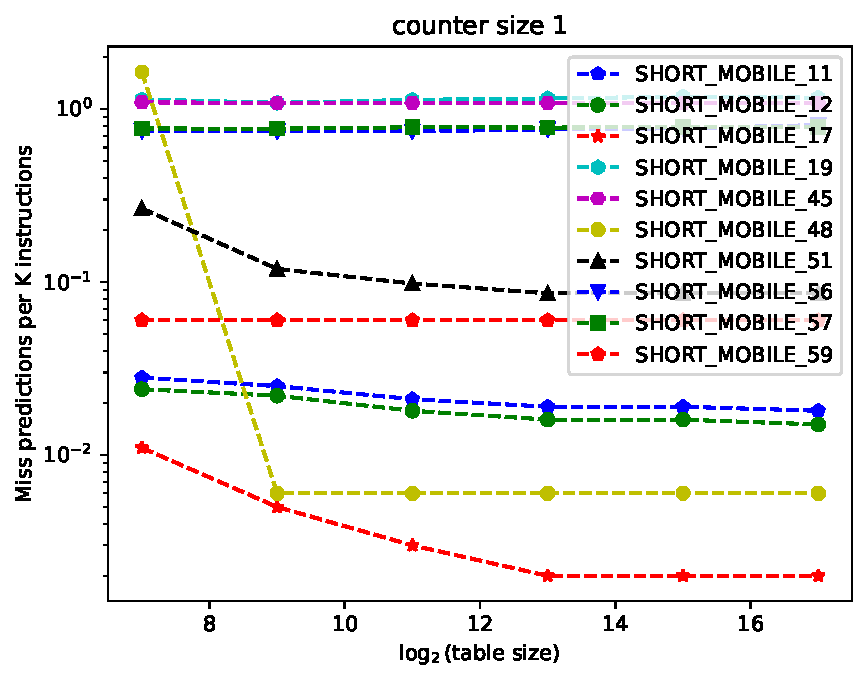
\includegraphics[width=\linewidth]{graph_1}
\end{minipage}%
\hfill
\begin{minipage}{.48\linewidth}
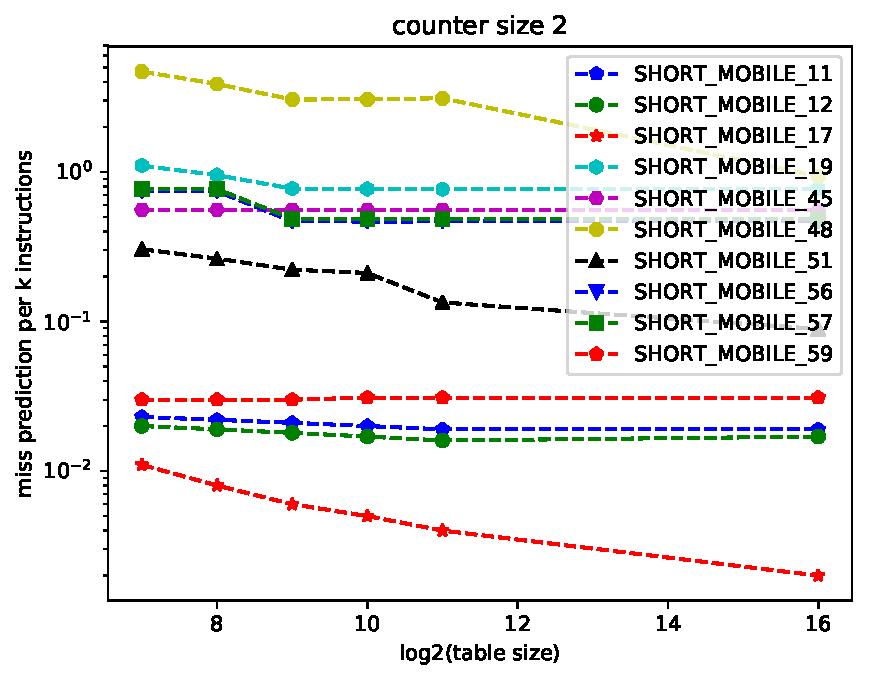
\includegraphics[width=\linewidth]{graph_2}
\end{minipage}

\begin{minipage}{.48\linewidth}
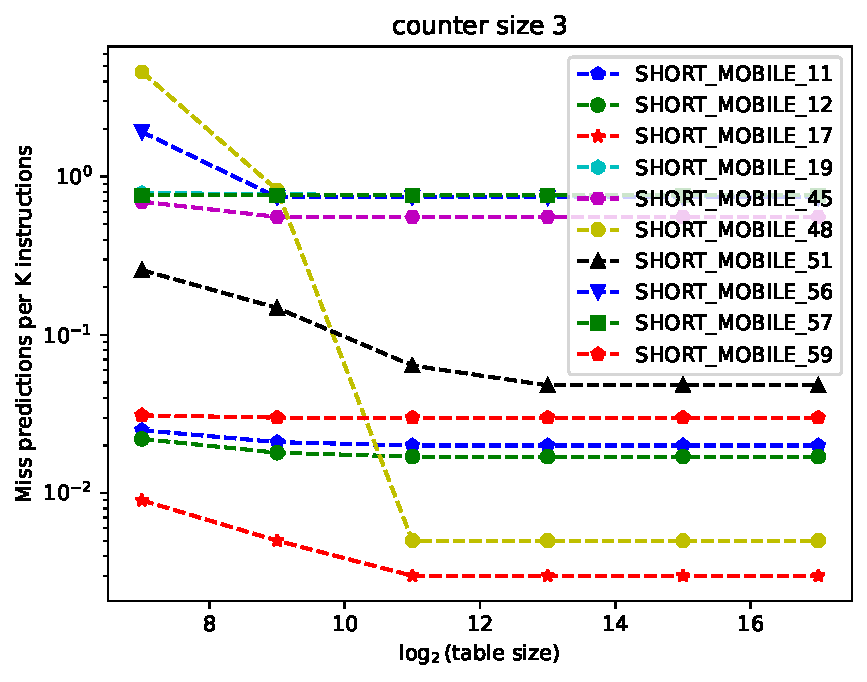
\includegraphics[width=\linewidth]{graph_3}
\end{minipage}%
\hfill
\begin{minipage}{.48\linewidth}
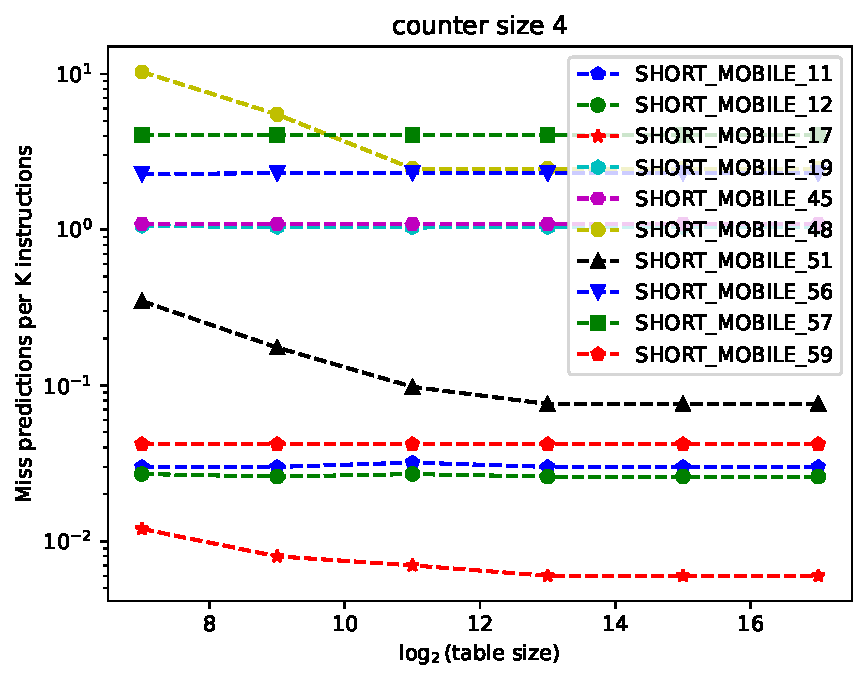
\includegraphics[width=\linewidth]{graph_4}
\end{minipage}

\begin{minipage}{.48\linewidth}
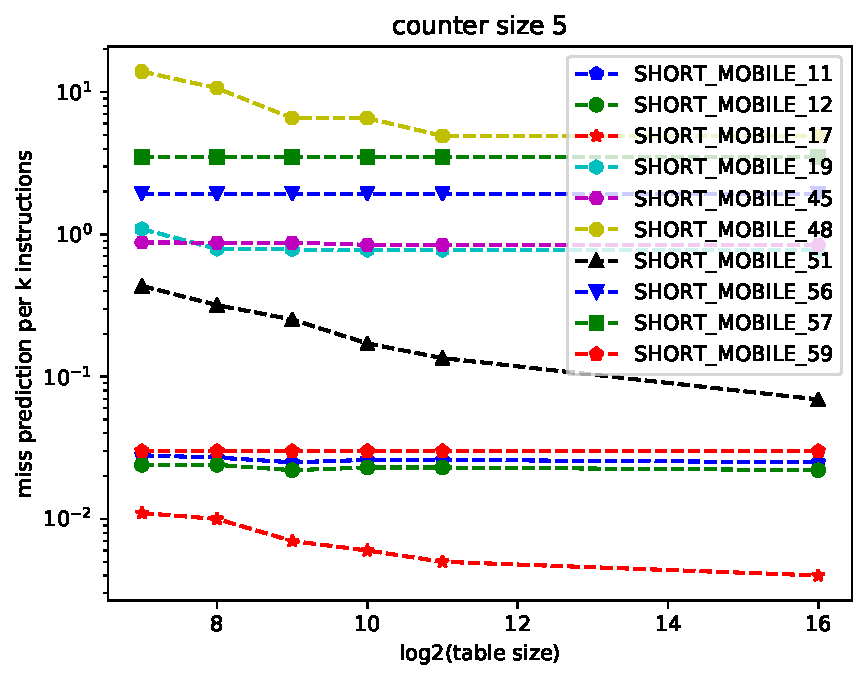
\includegraphics[width=\linewidth]{graph_5}
\end{minipage}%
\hfill
\begin{minipage}{.48\linewidth}
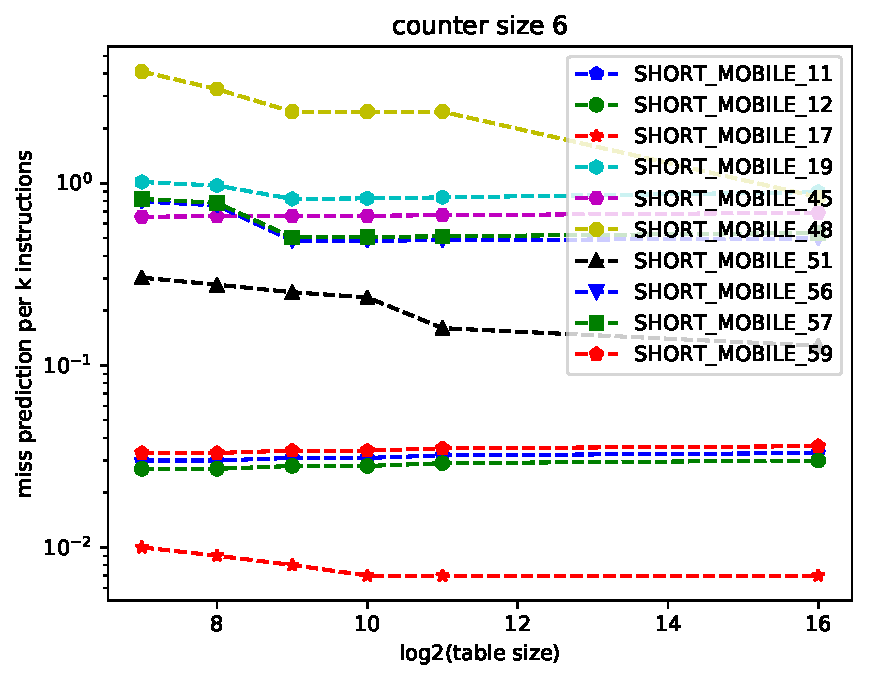
\includegraphics[width=\linewidth]{graph_6}
\end{minipage}
\subsection{Analyse}
On voit une asymptote due à la disparition des collisions lorsque la taille du prédicteur augmente.
Le coût du prédicteur est linéaire avec la taille du tableau, et il n'est pas raisonnable de dépasser $2^{16}$ éléments, d'autant que le gain à partir de $2^{12}$ devient très faible.
Par ailleurs, il y a toujours moins de $7\%$ de mauvaise prédictions, ce qui est remarquable pour une approche aussi simpliste.
\end{document}
